\chapter{The Two Diagnostic Technologies}
\label{ch:methods}

The diagnosis is a composition of two maps.
The first map, VWC, sends a triaxial acceleration record to a point in \(\R^{22}\).
The second map, MSFLA-SVM, sends that point to one of four labels, after a search has fixed the two parameters of a radial-basis support vector machine.
This chapter specifies both maps at the level of equations, algorithms, and implementation choices.
Where the source study leaves a choice unspecified, the choice is stated and marked as a specification of this exposition rather than as a recovered experimental setting.

\section{Technology one: the VWC feature map}
\label{sec:vwc}

\subsection{What the map is required to preserve}

Let one observation be three finite sequences
\begin{equation}
a_{r}[n],\ a_{t}[n],\ a_{a}[n],\qquad n=0,\ldots,N-1,
\label{eq:triaxial}
\end{equation}
sampled at \(f_{s}\), together with the shaft speed \(n_{\mathrm{rpm}}\) that fixes \(f_{0}\) through \eqref{eq:f0}.
On the published rig, \(f_{s}=10\,\mathrm{kHz}\), \(N=8192\), and \(n_{\mathrm{rpm}}=960\).
The map
\begin{equation}
\Phi:\ (a_{r}, a_{t}, a_{a})\ \longmapsto\ \vect{x}\in\R^{22}
\label{eq:phi}
\end{equation}
has to preserve three different facts at once.
The first fact is how hard the machine is vibrating, in the standardized sense of root-mean-square velocity.
The second fact is how that vibration is spread across time scales, so that a short-lived transient is not averaged into invisibility.
The third fact is how the energy of the loudest scale is distributed among the seven shaft orders in \eqref{eq:family}, because those orders are the mechanical vocabulary of the four states.
VWC is the conjunction of those three facts: vibration severity, the dyadic wavelet energy time-spectrum, and the coefficient power spectrum of the maximum-energy level.
The initial letters of the three blocks name the map.

The blocks are complementary in a precise sense.
Severity is invariant to a redistribution of energy among frequencies, which is why the pedestal fault hides inside it.
The energy time-spectrum is invariant to a redistribution among frequencies that share a scale, which is why two different shaft orders inside one dyadic band produce the same \(E_{j}\).
The coefficient power spectrum breaks that remaining invariance, at the price of being computed on only one scale.
Using the maximum-energy scale concentrates the third block where the record actually has energy, instead of averaging a spectrum over scales that contain only the noise floor.

\subsection{Vibration severity}

The continuous definition \eqref{eq:vibcont} and the discrete RMS \eqref{eq:vibdisc} are the first block.
The velocity series that enters \eqref{eq:vibdisc} is obtained from acceleration.
This exposition distinguishes the source formula from the integrator used to scale the illustrative figures.

The source formula accumulates absolute acceleration over a window of \(10\,\mathrm{ms}\),
\begin{equation}
v_{i}=\int_{0}^{0.01}\abs{a_{i}(t)}\,\mathrm{d}t.
\label{eq:vsrc}
\end{equation}
On a uniform grid with step \(\Delta t=1/f_{s}\) the integral is a sum of \(0.01 f_{s}\) samples.
At \(10\,\mathrm{kHz}\) that is \(100\) samples.
The absolute value makes \(v_{i}\) nonnegative and proportional to the local mean absolute acceleration.
Substituting the resulting series into \eqref{eq:vibdisc} produces the severity that the source reports: \(1.051\,\mathrm{mm/s}\) healthy, \(3.737\,\mathrm{mm/s}\) for the eccentric axle, \(1.161\,\mathrm{mm/s}\) for the bearing pedestal, and \(1.70024\,\mathrm{mm/s}\) for sealing-ring wear, all quoted for the radial direction in which the time-domain figures of the source are drawn.
Figure~\ref{fig:severity} restates those four numbers.
The eccentric state is more than three times the healthy severity.
The pedestal state is about ten percent above healthy.
A threshold on severity alone can flag the eccentric axle and cannot reliably flag the pedestal.

\begin{figure}[H]
\centering
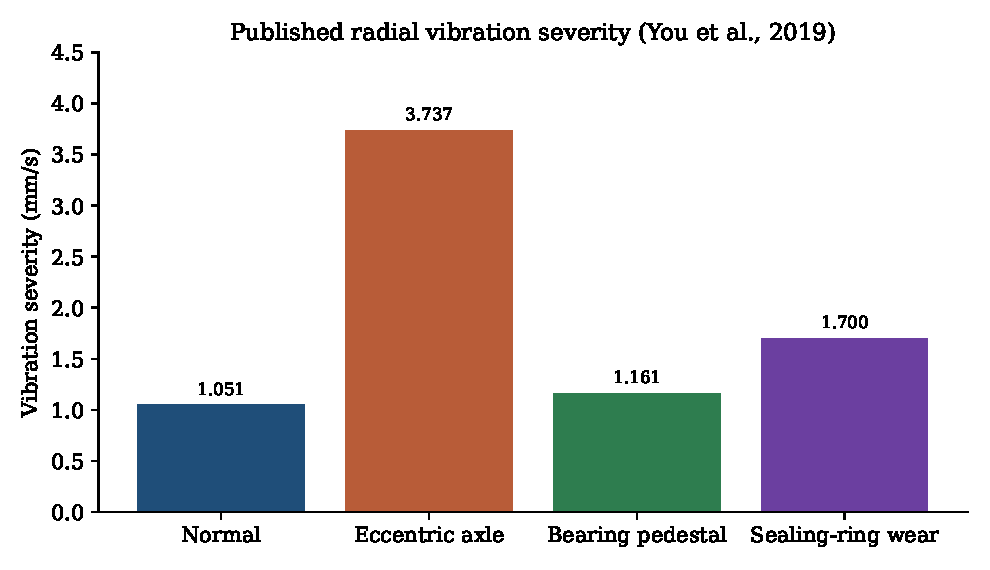
\includegraphics[width=0.78\textwidth]{severity.pdf}
\caption{Radial vibration severity reported by You et al.\ for the four operating states. These are published measurements, not quantities computed from the illustrative signals.}
\label{fig:severity}
\end{figure}

The illustrative waveforms of Figure~\ref{fig:waves} are built differently, and the difference is intentional.
Each synthetic acceleration is high-pass integrated,
\begin{equation}
\tilde{v}[n]=\Delta t\sum_{k=0}^{n} a[k],\qquad
v=\mathcal{H}_{2\,\mathrm{Hz}}\{\tilde{v}\},
\label{eq:illustvel}
\end{equation}
and the acceleration is scaled by a single positive constant until \(\sqrt{\tfrac{1}{N}\sum v[n]^{2}}\), expressed in millimetres per second, equals the published severity of that state.
The shape of each record---a shaft-locked fundamental, a half-order where the source describes one, a blade-pass component, a weak supply tone in the healthy state, and a resonance near \(200\,\mathrm{Hz}\) that gives the dyadic bank something to localize---follows the qualitative signatures of Section~\ref{sec:signatures}.
The samples are not a reconstruction of the laboratory series, whose raw values are not in the source paper.
They exist so that the later formulae can be looked at on a signal whose intensity and whose harmonic emphasis agree with the published description.

\begin{figure}[H]
\centering
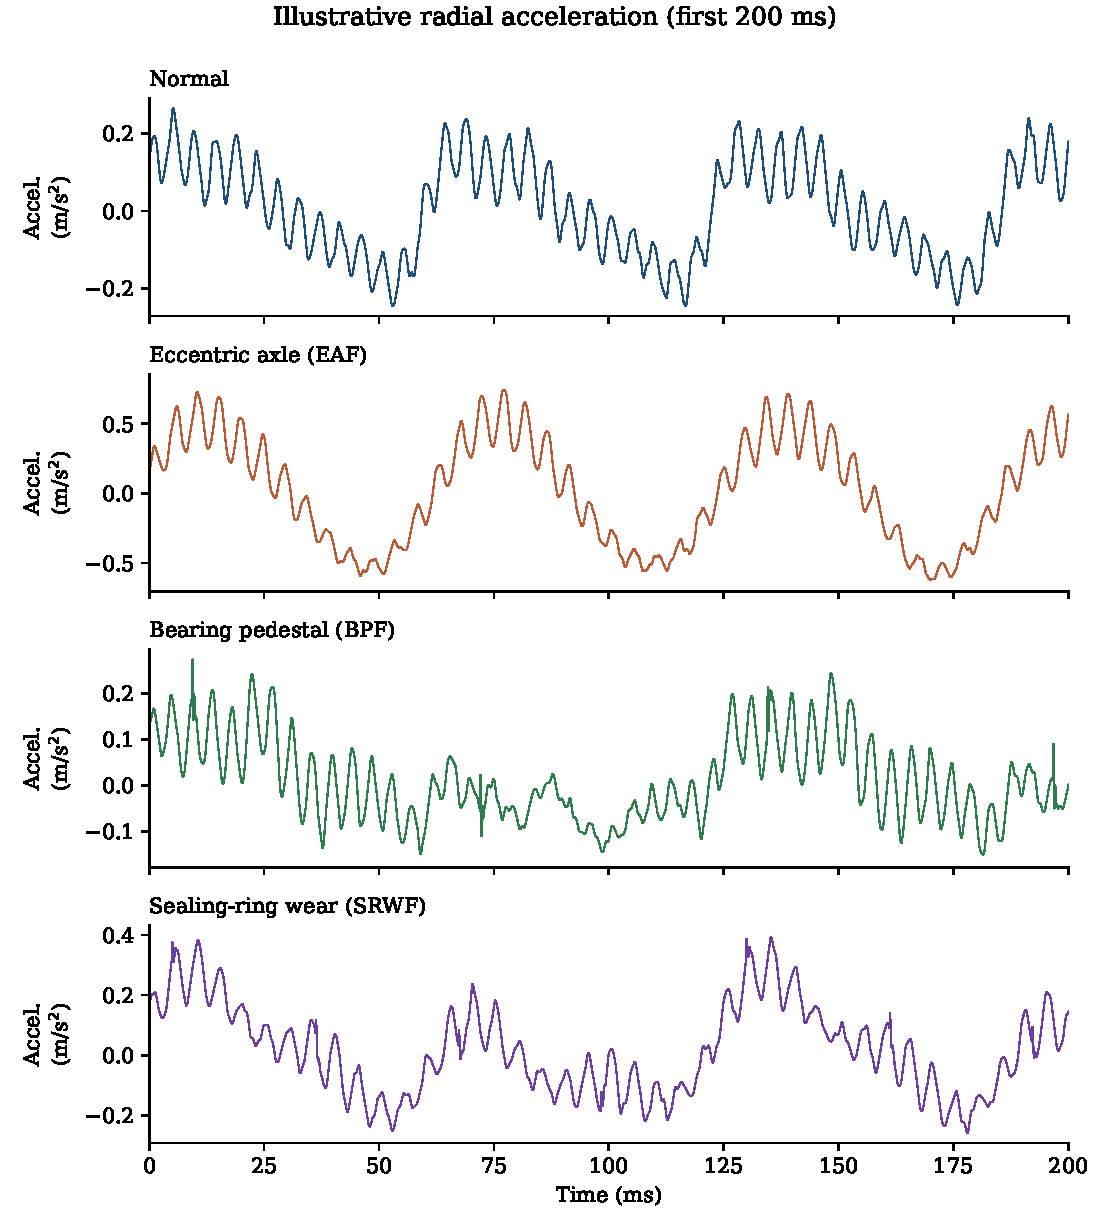
\includegraphics[width=0.92\textwidth]{waveforms.pdf}
\caption{Illustrative radial acceleration over the first \(200\,\mathrm{ms}\). Each record is scaled so that the RMS of its high-pass-integrated velocity equals the published severity of that state.}
\label{fig:waves}
\end{figure}

Severity contributes one coordinate to \(\vect{x}\), not three.
The arithmetic of the source is explicit: seven harmonics in three directions give \(21\) spectral coordinates, and the full vector has dimension \(22\), so exactly one severity is appended.
Figure~8 of the source shows that coordinate in the radial direction across groups of records.
This exposition takes the radial severity as that coordinate, because that is the direction for which a number is published, and it keeps the three-axis diversity for the spectral block where the source says the three axes differ.

\subsection{The dyadic wavelet and the Mallat bank}

The second block begins with a mother wavelet \(\psi\in L^{2}(\R)\) of zero mean and unit norm.
The dyadic family at scale \(2^{j}\) and translation \(b\) is
\begin{equation}
\psi_{2^{j}, b}(t)=2^{-j/2}\,\psi\bigl(2^{-j}(t-b)\bigr),\qquad j\in\mathbb{Z}.
\label{eq:dyadic}
\end{equation}
The factor \(2^{-j/2}\) keeps the \(L^{2}\) norm equal to one for every \(j\).
The analysis formula used by the source is the inner product
\begin{equation}
W_{f}(2^{j}, b)=2^{-j/2}\int_{-\infty}^{\infty} f(t)\,\psi^{*}\bigl(2^{-j}(t-b)\bigr)\,\mathrm{d}t
=\bigl(f*\overline{\psi}_{2^{j}}\bigr)(b),
\label{eq:wt}
\end{equation}
with \(\overline{\psi}_{2^{j}}(u)=\psi_{2^{j}}(-u)\).
On a sampled record the inner product is not computed as an integral.
It is computed by the filter bank \eqref{eq:mallat}, which Mallat showed to be equivalent to \eqref{eq:wt} when \(\psi\) is the wavelet of a multiresolution analysis.

One step of that bank is drawn in Figure~\ref{fig:mallat}.
The approximation coefficients at level \(j-1\) are convolved with the low-pass analysis filter \(h\) and with the high-pass analysis filter \(g\), and both results are downsampled by two.
The downsampled high-pass branch is the detail \(cD^{j}\).
The downsampled low-pass branch is the approximation \(cA^{j}\), which becomes the input of level \(j+1\).
Reconstruction, written by the source as
\begin{equation}
cA^{j-1}[k]=\sum_{n} cA^{j}[n]\,h[k-2n]+\sum_{n} cD^{j}[n]\,g[k-2n],
\label{eq:recon}
\end{equation}
is the identity that lets a detail be put back into the original sampling grid and inspected as a time series.
Orthonormal filter pairs satisfy a quadrature mirror relation, so the sum of detail energies and the final approximation energy equals the energy of the input, up to the boundary treatment.
That identity is what makes a bar chart of energy-by-level a partition of the record rather than an arbitrary scoring.

\begin{figure}[H]
\centering
\begin{tikzpicture}[
  blk/.style={draw, minimum width=16mm, minimum height=7mm, font=\small, align=center},
  arr/.style={-{Stealth[length=2mm]}, thick},
  ds/.style={draw, circle, inner sep=1pt, font=\scriptsize, minimum size=6mm}
]
\node[blk, fill=blue!8] (in) {\(cA^{j-1}\)};
\node[blk, fill=orange!15, right=8mm of in] (lo) {\(h\)\\low-pass};
\node[blk, fill=orange!15, below=6mm of lo] (hi) {\(g\)\\high-pass};
\node[ds, right=8mm of lo] (ds1) {\(\downarrow 2\)};
\node[ds, right=8mm of hi] (ds2) {\(\downarrow 2\)};
\node[blk, fill=green!10, right=8mm of ds1] (a) {\(cA^{j}\)};
\node[blk, fill=green!10, right=8mm of ds2] (d) {\(cD^{j}\)};
\draw[arr] (in) -- (lo);
\draw[arr] (in.south) |- (hi.west);
\draw[arr] (lo) -- (ds1);
\draw[arr] (hi) -- (ds2);
\draw[arr] (ds1) -- (a);
\draw[arr] (ds2) -- (d);
\node[font=\scriptsize, align=left, below=2mm of d] {detail energy \(E_{j}=\norm{cD^{j}}^{2}\)};
\end{tikzpicture}
\caption{One step of the Mallat analysis bank. The detail coefficients at level \(j\) are the dyadic wavelet transform at scale \(2^{j}\).}
\label{fig:mallat}
\end{figure}

This exposition uses the Daubechies wavelet with four vanishing moments (db4) as the concrete mother wavelet.
The source does not name the mother wavelet.
Db4 is short, orthonormal, and has enough vanishing moments to annihilate a local cubic trend, which is the usual default when a monitoring study leaves the wavelet unnamed.
The analysis filters used to draw Figure~\ref{fig:energy} are the standard db4 pair.
A change to db6 or to a symlet moves the energy slightly between neighboring levels and does not change the definition of the map.
The level index, however, must be read against the sampling rate.
With \(f_{s}=10\,\mathrm{kHz}\), ideal dyadic half-bands place detail \(d_{j}\) roughly in
\begin{equation}
\Bigl(\frac{f_{s}}{2^{j+1}},\ \frac{f_{s}}{2^{j}}\Bigr).
\label{eq:bands}
\end{equation}
Detail \(d_{5}\) then occupies about \(156\)--\(312\,\mathrm{Hz}\), detail \(d_{6}\) about \(78\)--\(156\,\mathrm{Hz}\), and the shaft family \(\mathcal{F}\) itself, from \(8\,\mathrm{Hz}\) to \(96\,\mathrm{Hz}\), falls in \(d_{7}\), \(d_{8}\), and the final approximation.
The source figures identify \(d_{5}\) as the maximum-energy detail of the records they plot.
That observation is consistent with a structural or fluid resonance in the few-hundred-hertz band carrying more acceleration energy than the shaft tones, which is exactly what the factor \(-\omega^{2}\) in \eqref{eq:transfer} predicts.
The coefficient spectrum can still show shaft orders, because those orders modulate the resonant carrier, and because the spectrum the source plots is a spectrum of the selected detail's coefficient sequence with a frequency axis returned to hertz.
Both effects are part of the third block.

\begin{figure}[H]
\centering
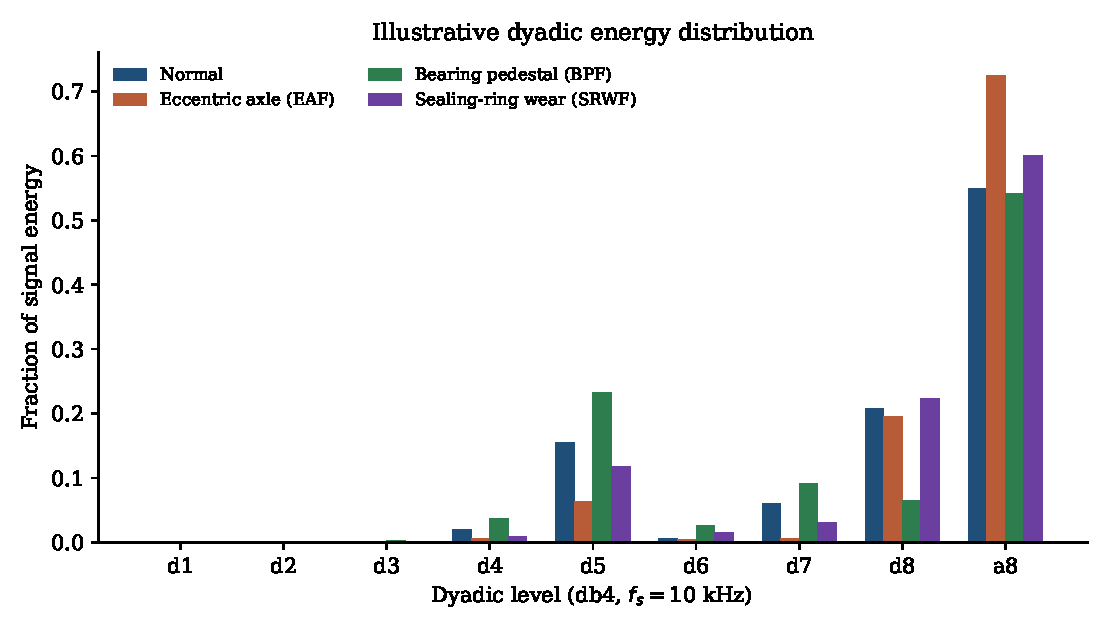
\includegraphics[width=0.92\textwidth]{wavelet_energy.pdf}
\caption{Fraction of energy by dyadic level for the illustrative signals, db4, eight levels. The bars are a partition of each synthetic record. They are not the energy table of the laboratory records, which the source publishes only as plots.}
\label{fig:energy}
\end{figure}

\subsection{Energy time-spectrum}

The source identifies the detail coefficients with the dyadic transform,
\begin{equation}
W_{f}(2^{j}, b)=cD^{j}[k],
\label{eq:identify}
\end{equation}
and defines the energy time-spectrum at scale \(2^{j}\) by the squared coefficients
\begin{equation}
E_{W_{f}(t)}(2^{j})=\abs{W_{f}(2^{j}, b)}^{2}=\abs{cD^{j}[k]}^{2}.
\label{eq:ets}
\end{equation}
Read as a function of the coefficient index, \eqref{eq:ets} is a time series, not a scalar.
It shows when, inside the record, scale \(2^{j}\) was loud.
A pedestal impact that occupies one millisecond raises \(E\) at the fine scales for that millisecond and leaves the rest of the series small.
A steady unbalance raises the coarse-scale series almost uniformly.
The scalar energy of the level, which decides the maximum, is the sum of the time series,
\begin{equation}
\mathcal{E}(2^{j})=\sum_{k}\abs{cD^{j}[k]}^{2}=\sum_{k} E_{W_{f}(t)}(2^{j})[k].
\label{eq:sumE}
\end{equation}
The maximum-energy level is the integer
\begin{equation}
k^{\star}\in\argmin_{1\le j\le J}\bigl(-\mathcal{E}(2^{j})\bigr),
\label{eq:kstar}
\end{equation}
that is, any level whose scalar energy is largest.
The source writes the assumption \(1\le k\le j\) for this index.
Ties are broken by choosing the finer level, so that a transient is preferred over a trend of equal energy.
On the source plots, \(k^{\star}=5\) for the displayed radial records of every state.
The map does not hard-code the number \(5\).
It recomputes \(k^{\star}\) for each record and each direction.
A fixed level would be a different method.

\subsection{Coefficient power spectrum of the maximum-energy level}

The third block reads the internal periodicity of the winning level.
The source forms the discrete Fourier transform of the energy time-series at \(k^{\star}\),
\begin{equation}
\widehat{E}_{W_{f}}(2^{k^{\star}})[\omega]
=\sum_{n=0}^{N_{c}-1} E_{W_{f}(t)}(2^{k^{\star}})[n]\,e^{-i\omega n/N_{c}},
\label{eq:fftE}
\end{equation}
and the power spectrum
\begin{equation}
E_{W_{p}}(\hat{\omega}, 2^{k^{\star}})
=\frac{1}{N_{c}}\left|\widehat{E}_{W_{f}}(2^{k^{\star}})[\omega]\right|^{2}.
\label{eq:cps}
\end{equation}
Here \(N_{c}\) is the length of the coefficient sequence at that level, which is about \(N/2^{k^{\star}}\) for an undecimated-free dyadic bank.
Equation \eqref{eq:cps} is the power spectrum of the energy envelope of the winning detail.
Peaks of an energy envelope sit at the rates that modulate the detail: a once-per-revolution modulation produces a line at \(f_{0}\) in this spectrum, and a twice-per-revolution looseness produces a line at \(\tfrac12 f_{0}\).

The plots in the source are labeled as the wavelet coefficient power spectrum of level \(d_{5}\) and are drawn with a horizontal axis in hertz from \(0\) to about \(110\,\mathrm{Hz}\), with visible lines at members of \(\mathcal{F}\).
Two implementations produce a plot of that shape.
The first is literal: transform \eqref{eq:ets} by \eqref{eq:fftE}, convert the coefficient-domain frequency \(\nu\) (cycles per coefficient) into hertz by
\begin{equation}
f=\nu\cdot\frac{f_{s}}{2^{k^{\star}}},
\label{eq:fmap}
\end{equation}
and read \eqref{eq:cps} on \(\mathcal{F}\).
The second forms the power spectrum of the detail coefficients themselves, without the square inside \eqref{eq:ets}, and uses the same frequency map.
The square emphasizes the strong instants of the detail and is the formula the source writes.
This exposition follows the written formula.
Amplitudes at the seven orders are then the samples of \eqref{eq:cps} nearest to each frequency in \(\mathcal{F}\),
\begin{equation}
p_{d}(\eta)=\left. E_{W_{p}}(\hat{\omega}, 2^{k^{\star}}) \right|_{f=\eta},
\qquad \eta\in\mathcal{F},\quad d\in\{r, t, a\}.
\label{eq:samples}
\end{equation}
If a line falls between bins, the bin of maximum power inside a window of half a shaft order is taken, so that a \(1\,\mathrm{Hz}\) speed drift does not zero the feature.
The source does not describe an interpolation rule.
The half-order window is a specification of this exposition, and it is narrower than the gap between adjacent members of \(\mathcal{F}\).

Figure~\ref{fig:spectra} shows the baseband power of the illustrative accelerations, normalized per state, with vertical lines at the same orders.
It is a spectrum of the raw synthetic signal, included so the harmonic emphasis is visible without the filter bank.
It is not a plot of \eqref{eq:cps}.

\begin{figure}[H]
\centering
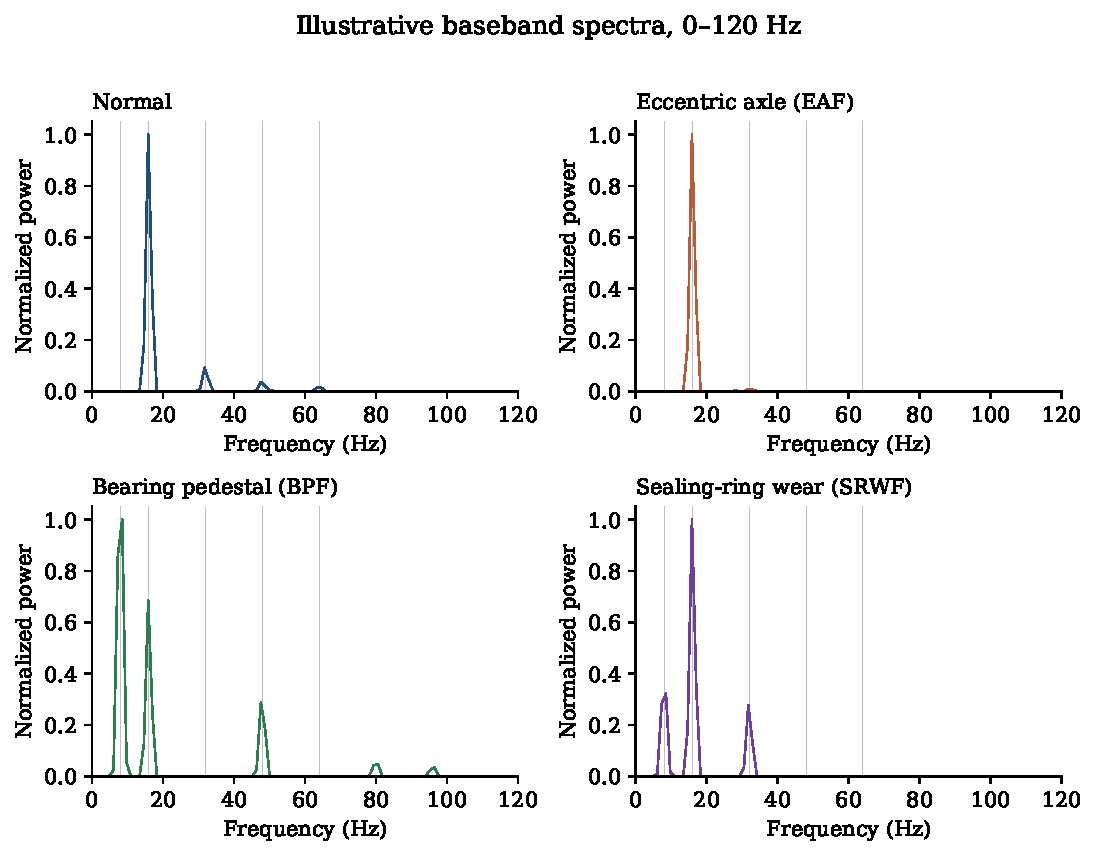
\includegraphics[width=0.94\textwidth]{spectra.pdf}
\caption{Normalized baseband spectra of the illustrative accelerations. Vertical lines mark \(8\), \(16\), \(32\), \(48\), and \(64\,\mathrm{Hz}\). Healthy energy favors \(f_{0}\) and its low harmonics; the eccentric state is dominated by \(f_{0}\); the pedestal and seal-wear states carry a stronger half-order.}
\label{fig:spectra}
\end{figure}

\subsection{Assembly of the twenty-two coordinates}

Collect the seven spectral samples on each axis and the radial severity:
\begin{equation}
\begin{aligned}
\vect{x}=\bigl(&
\mathrm{VIB}_{r},\\
&p_{t}(\tfrac12 f_{0}), p_{t}(f_{0}), \ldots, p_{t}(6f_{0}),\\
&p_{a}(\tfrac12 f_{0}), p_{a}(f_{0}), \ldots, p_{a}(6f_{0}),\\
&p_{r}(\tfrac12 f_{0}), p_{r}(f_{0}), \ldots, p_{r}(6f_{0})
\bigr)^{\!\top}\in\R^{22}.
\end{aligned}
\label{eq:x22}
\end{equation}
The order of the blocks is a convention.
Training and testing must use the same convention, because the SVM kernel compares coordinates by index.
The source's reading of its own Figure~9 fixes the meaning of the blocks even without a written index map.
In the healthy state the tangential amplitudes exceed the axial and the radial ones, and the tangential maximum lies at \(f_{0}\).
Under the eccentric axle the tangential maximum rises from \(1.683\times 10^{-3}\) to \(3.322\times 10^{-3}\) in the units of that figure, the axial energy spreads from \(f_{0}\) toward \(\tfrac12 f_{0}\), and the radial maximum rises from \(4.574\times 10^{-4}\) to \(2.492\times 10^{-3}\).
Under the pedestal fault the tangential maximum rises further, to \(4.701\times 10^{-3}\), and it sits at \(\tfrac12 f_{0}\) rather than at \(f_{0}\); axial energy grows at \(5f_{0}\) and \(6f_{0}\); radial energy shifts from \(f_{0}\) toward \(\tfrac12 f_{0}\), \(3f_{0}\), and \(4f_{0}\).
Under sealing-ring wear the tangential amplitudes are again the largest, with emphasis at \(f_{0}\), \(\tfrac12 f_{0}\), and \(2f_{0}\), and the axial and radial intensities fall between the eccentric and the pedestal cases.
Those sentences are the specification of what \(\Phi\) is supposed to make linearly visible.
A correct implementation is one in which a scatter of the \(22\)-vectors reproduces this pattern.

\subsection{Normalization}

Coordinates of \(\vect{x}\) do not share a unit.
Severity is in millimetres per second and has magnitude near \(1\).
A coefficient power sample is a squared spectral density of a squared wavelet coefficient, and the published tangential peaks lie near \(10^{-3}\).
Left unscaled, the Euclidean distances inside the radial kernel are severity distances, and the twenty-one spectral coordinates are ignored.
The source states that training and testing vectors are normalized before classification in order to speed convergence.
It does not state the map.
This exposition uses an affine map to the unit interval, fit on the training sample only,
\begin{equation}
\tilde{x}^{(j)}=\frac{x^{(j)}-u^{(j)}}{v^{(j)}-u^{(j)}},
\qquad
u^{(j)}=\min_{i\in\mathrm{train}} x_{i}^{(j)},
\quad
v^{(j)}=\max_{i\in\mathrm{train}} x_{i}^{(j)}.
\label{eq:norm}
\end{equation}
The same \(u^{(j)}\) and \(v^{(j)}\) are applied to the test vectors.
Refitting the range on the test set would leak the test distribution into the feature and would inflate the estimate in Chapter~\ref{ch:estimation}.
A coordinate with \(v^{(j)}=u^{(j)}\) is dropped; on this rig none of the twenty-two is constant.
A \(z\)-score is an acceptable alternative and is not the map used in the formulae below.

\subsection{The feature procedure}

The map \(\Phi\), ready to implement, is the following procedure.
\begin{enumerate}
\item From each acceleration axis, form the velocity series by the chosen integrator and compute one radial severity by \eqref{eq:vibdisc}.
\item For each axis, run \(J=8\) steps of \eqref{eq:mallat} with the db4 filters.
Compute the scalar energies \eqref{eq:sumE} and the winning index \(k^{\star}\) by \eqref{eq:kstar}.
\item Form the energy time-series \eqref{eq:ets} at level \(k^{\star}\), its transform \eqref{eq:fftE}, and the power \eqref{eq:cps}.
Sample the seven orders by \eqref{eq:samples}.
\item Concatenate by \eqref{eq:x22}.
\item Apply \eqref{eq:norm} with ranges stored from the training fold.
\end{enumerate}
The cost is linear in \(N\) for the filter bank and \(O(N_{c}\log N_{c})\) for the single transform of the winning level.
At \(N=8192\) this cost is negligible beside the cost of the SVM trainings inside the parameter search.
The map contains no iterative optimization and no random seed.
Given the filter, the integrator, and the tie break, \(\Phi\) is a function.

\subsection{How the four states separate inside the map}

A short mechanical reading says what a later classifier is asked to finish.
Healthy running puts a moderate severity next to a tangential spectrum peaked at \(16\,\mathrm{Hz}\), with smaller lines at \(32\), \(48\), and \(64\,\mathrm{Hz}\) and a supply artifact at \(50\,\mathrm{Hz}\) that the order sampler, aimed at \(48\,\mathrm{Hz}\), is narrow enough to miss.
Eccentric axle multiplies the severity by about three and multiplies the tangential \(f_{0}\) sample by about two, which is the stationary signature of a larger \(me\Omega^{2}\) in \eqref{eq:rotor}.
Bearing-pedestal fault leaves the severity almost unchanged and moves the tangential peak from \(16\,\mathrm{Hz}\) to \(8\,\mathrm{Hz}\), which is the spectral form of a stiffness that repeats every two revolutions, and it raises high-order axial energy that the source attributes to flow-induced vibration and to component natural frequencies.
Sealing-ring wear raises the severity to \(1.70\,\mathrm{mm/s}\) and emphasizes \(\tfrac12 f_{0}\) together with \(2f_{0}\), which is the hydraulic leakage writing on the orbit twice per turn as well as once every two turns.
These four patterns are not orthogonal, and the pedestal pattern is the least stable of them because resonance and site interference share the bands the high orders occupy.
The classifier of the next section is trained to draw the boundaries that these patterns only suggest.

\begin{figure}[H]
\centering
\begin{tikzpicture}[
  box/.style={draw, rounded corners=2pt, align=center, font=\small, inner sep=3pt, minimum height=8mm},
  arr/.style={-{Stealth[length=2mm]}, thick}
]
\node[box, fill=blue!8, text width=26mm] (a) {Triaxial\\acceleration};
\node[box, fill=orange!12, text width=28mm, right=5mm of a] (v) {Radial severity\\\eqref{eq:vibdisc}};
\node[box, fill=orange!12, text width=32mm, below=5mm of v] (w) {Mallat bank\\energies \(\mathcal{E}(2^{j})\)};
\node[box, fill=orange!12, text width=34mm, right=5mm of w] (c) {CPS at \(k^{\star}\)\\seven orders, three axes};
\node[box, fill=green!12, text width=24mm, right=5mm of v] (x) {\(\vect{x}\in\R^{22}\)};
\node[box, fill=green!12, text width=24mm, right=5mm of x] (n) {Train-only\\scaling \eqref{eq:norm}};
\draw[arr] (a) -- (v);
\draw[arr] (a.south) ++(0,-1mm) |- (w.west);
\draw[arr] (w) -- (c);
\draw[arr] (v) -- (x);
\draw[arr] (c.north) |- (x.south);
\draw[arr] (x) -- (n);
\end{tikzpicture}
\caption{Data flow of the VWC map. Severity and the spectral block meet only at the concatenation.}
\label{fig:vwcflow}
\end{figure}

\section{Technology two: the MSFLA-SVM classifier}
\label{sec:svm}

\subsection{Hard margin}

The second technology starts from a binary labeled sample, because the multiclass pump problem is reduced to binary problems below.
Let
\begin{equation}
\mathcal{T}=\bigl\{(\vect{x}_{i}, y_{i})\bigr\}_{i=1}^{n},
\qquad \vect{x}_{i}\in\R^{d},\quad y_{i}\in\{+1,-1\}.
\label{eq:binset}
\end{equation}
A linear classifier is a pair \((\vect{w}, b)\) and the rule \(\sgn(\vect{w}^{\top}\vect{x}+b)\).
Among all pairs that separate \(\mathcal{T}\), the hard-margin SVM chooses the pair whose slab
\begin{equation}
\bigl\{\vect{x}:\ \abs{\vect{w}^{\top}\vect{x}+b}\le 1\bigr\}
\label{eq:slab}
\end{equation}
is as thick as possible.
The Euclidean thickness of the slab is \(2/\norm{\vect{w}}\).
Maximizing the thickness is the same problem as
\begin{equation}
\min_{\vect{w}, b}\ \frac{1}{2}\norm{\vect{w}}^{2}
\quad\text{subject to}\quad
y_{i}(\vect{w}^{\top}\vect{x}_{i}+b)\ge 1,
\quad i=1,\ldots,n.
\label{eq:hard}
\end{equation}
The factor one half is traditional and makes the derivative equal to \(\vect{w}\).
Points that lie on the boundary of the slab are the support vectors.
They alone determine \(\vect{w}\).
Moving a correctly classified point that sits strictly outside the slab does not change the solution, which is the geometric reason a small sample can still determine a stable rule: most of the sample is allowed to be absent.

\begin{figure}[H]
\centering
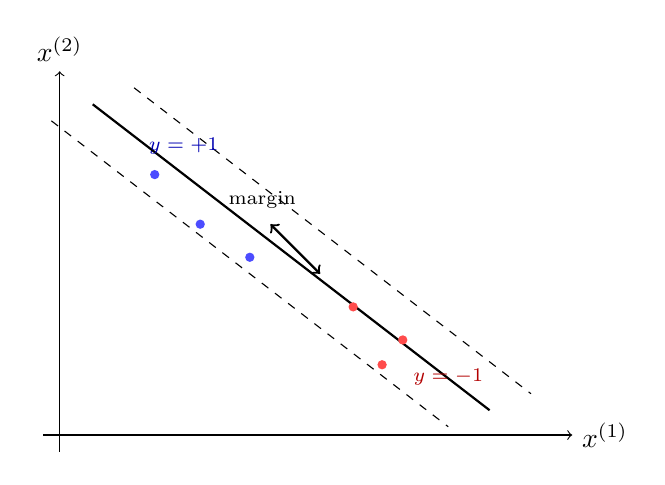
\begin{tikzpicture}[scale=1.05]
  \draw[->] (-0.2,0) -- (6.2,0) node[right] {\(x^{(1)}\)};
  \draw[->] (0,-0.2) -- (0,4.4) node[above] {\(x^{(2)}\)};
  \draw[thick] (0.4,4.0) -- (5.2,0.3);
  \draw[dashed] (0.9,4.2) -- (5.7,0.5);
  \draw[dashed] (-0.1,3.8) -- (4.7,0.1);
  \fill[blue!70] (1.15,3.15) circle (1.6pt);
  \fill[blue!70] (1.7,2.55) circle (1.6pt);
  \fill[blue!70] (2.3,2.15) circle (1.6pt);
  \fill[red!70] (3.55,1.55) circle (1.6pt);
  \fill[red!70] (4.15,1.15) circle (1.6pt);
  \fill[red!70] (3.9,0.85) circle (1.6pt);
  \draw[<->, thick] (2.55,2.55) -- (3.15,1.95);
  \node[font=\scriptsize] at (2.45,2.85) {margin};
  \node[font=\scriptsize, blue!70!black] at (1.5,3.5) {\(y=+1\)};
  \node[font=\scriptsize, red!70!black] at (4.7,0.7) {\(y=-1\)};
\end{tikzpicture}
\caption{Hard-margin geometry in a feature plane. The solid line is the decision boundary. The dashed lines bound the slab. Only points on the dashed lines are support vectors.}
\label{fig:margin}
\end{figure}

\subsection{Soft margin and the dual}

Pump features overlap, so the constraints of \eqref{eq:hard} can be empty.
The soft-margin problem introduces a slack \(\xi_{i}\ge 0\) for each training point and a penalty \(C>0\) on the sum of slacks,
\begin{equation}
\min_{\vect{w}, b, \xi}\ 
\frac{1}{2}\norm{\vect{w}}^{2}+C\sum_{i=1}^{n}\xi_{i}
\quad\text{subject to}\quad
y_{i}(\vect{w}^{\top}\vect{x}_{i}+b)\ge 1-\xi_{i},\quad \xi_{i}\ge 0.
\label{eq:soft}
\end{equation}
A small \(C\) permits a wide margin with many slacks and under-fits the four states.
A large \(C\) forces the slacks toward zero and can memorize the \(180\) training vectors.
This is the first of the two numbers the frog search has to set.
The Lagrangian of \eqref{eq:soft} with multipliers \(\alpha_{i}\ge 0\) for the margin inequalities and \(\mu_{i}\ge 0\) for the slack inequalities has a saddle point at which \(\vect{w}=\sum_{i}\alpha_{i} y_{i}\vect{x}_{i}\) and \(\sum_{i}\alpha_{i} y_{i}=0\).
Eliminating \(\vect{w}\), \(b\), and \(\xi\) produces the dual quadratic program that the source writes in kernel form.
In the linear case it is
\begin{equation}
\begin{aligned}
\max_{\alpha}\quad
&-\frac{1}{2}\sum_{i=1}^{n}\sum_{j=1}^{n} y_{i} y_{j}\alpha_{i}\alpha_{j}\,\vect{x}_{i}^{\top}\vect{x}_{j}
+\sum_{j=1}^{n}\alpha_{j}\\
\text{subject to}\quad
&\sum_{i=1}^{n} y_{i}\alpha_{i}=0,
\qquad 0\le \alpha_{i}\le C.
\end{aligned}
\label{eq:dual}
\end{equation}
The box constraint \(0\le\alpha_{i}\le C\) is the algebraic face of the penalty.
A point with \(\alpha_{i}=0\) is outside the slab and does not appear in \(\vect{w}\).
A point with \(0<\alpha_{i}<C\) lies on the margin boundary and is a free support vector.
A point with \(\alpha_{i}=C\) lies inside the slab or on the wrong side and is a bound support vector.
The decision rule, once any free support vector \(\vect{x}_{j}\) has been used to recover the threshold, is
\begin{equation}
f(\vect{x})=\sgn\Bigl(\sum_{i=1}^{n}\alpha_{i} y_{i}\,\vect{x}_{i}^{\top}\vect{x}+b\Bigr),
\label{eq:declin}
\end{equation}
\begin{equation}
b=y_{j}\Bigl(1-\frac{\alpha_{j}}{C}\Bigr)-\sum_{i=1}^{n} y_{i}\alpha_{i}\,\vect{x}_{i}^{\top}\vect{x}_{j},
\label{eq:bias}
\end{equation}
which is the linear special case of the source formulae.
Sequential minimal optimization solves \eqref{eq:dual} by optimizing two multipliers at a time and keeping the equality constraint satisfied.
The solver is deterministic given the data, \(C\), and the kernel.
All of the randomness in MSFLA-SVM sits in the outer search, not in the quadratic program.

\subsection{The radial kernel}

Pump classes are not linearly separable in \(\R^{22}\) after the normalization \eqref{eq:norm}.
A feature map \(\Psi\) into a Hilbert space \(\mathcal{H}\) restores a linear problem in \(\mathcal{H}\) provided the inner products \(\langle\Psi(\vect{x}),\Psi(\vect{x}')\rangle_{\mathcal{H}}\) can be evaluated.
Mercer's theorem says that a continuous symmetric function \(K\) that is positive definite is such an inner product for some \(\Psi\).
The radial basis used by the source,
\begin{equation}
K(\vect{x}, \vect{x}')
=\exp\Bigl(-\frac{\norm{\vect{x}-\vect{x}'}^{2}}{2\sigma^{2}}\Bigr)
=\exp\bigl(-g\,\norm{\vect{x}-\vect{x}'}^{2}\bigr),
\label{eq:rbf}
\end{equation}
is positive definite for every \(\sigma>0\).
The second writing defines the kernel parameter \(g=1/(2\sigma^{2})\) that the search actually stores.
A large \(g\) makes \(K\) decay in a small neighborhood of each training point: the decision surface can weave among the \(180\) vectors and the risk of over-fit rises.
A small \(g\) makes \(K\) almost constant on the unit cube: the surface is nearly linear and the risk of under-fit rises.
The source notes that \(\sigma\), or equivalently \(g\), balances the influence of \(C\).
The pair \((C, g)\) is the whole continuous degree of freedom of the classifier.
Substituting \(K\) for the inner product in \eqref{eq:dual} gives the program the source states,
\begin{equation}
\begin{aligned}
\min_{\alpha}\quad
&\frac{1}{2}\sum_{i=1}^{n}\sum_{j=1}^{n}
y_{i} y_{j}\alpha_{i}\alpha_{j}
\Bigl(K(\vect{x}_{i}, \vect{x}_{j})+\frac{1}{C}\delta_{ij}\Bigr)
-\sum_{j=1}^{n}\alpha_{j}\\
\text{subject to}\quad
&\sum_{i=1}^{n} y_{i}\alpha_{i}=0,\qquad \alpha_{i}\ge 0,
\end{aligned}
\label{eq:dualk}
\end{equation}
where the diagonal term \(C^{-1}\delta_{ij}\) is the source's way of writing the soft-margin quadratic, and the decision function is
\begin{equation}
f(\vect{x})=\sgn\Bigl(\sum_{i=1}^{n}\alpha_{i}^{\star} y_{i} K(\vect{x}, \vect{x}_{i})+b^{\star}\Bigr).
\label{eq:decf}
\end{equation}
The threshold \(b^{\star}\) is computed from any multiplier strictly between \(0\) and \(C\), by the kernel form of \eqref{eq:bias}.

\subsection{Four states from binary machines}

The label set of the pump is
\begin{equation}
\mathcal{Y}=\{\text{normal},\ \text{EAF},\ \text{BPF},\ \text{SRWF}\},
\label{eq:Y}
\end{equation}
not a pair.
This exposition reduces \(\mathcal{Y}\) by the one-versus-one scheme.
Each pair of states trains one binary machine, which produces
\begin{equation}
\binom{4}{2}=6
\label{eq:ovo}
\end{equation}
radial SVMs.
A test vector is labeled by the state that wins the most of the six votes.
Ties are broken by the signed sum of the six decision functions after each function has been oriented toward its positive class.
One-versus-rest, with four machines, is the main alternative.
It trains each machine on a more unbalanced binary problem, because the negative class then contains three states.
The source does not name the reduction.
One-versus-one is the specification here because each binary problem then has \(90\) training vectors, \(45\) per state, which matches the per-state training count the source publishes, and because it is the default reduction of the usual SVM solver.
The search for \((C, g)\) is shared: one pair is used for all six machines, and the fitness of that pair is the cross-validated accuracy of the voted label, not the accuracy of a single binary machine.
Searching six independent pairs would multiply the capacity of the outer loop by six and, on \(180\) vectors, would over-fit the folds.

\subsection{Cross-validated fitness}

A frog is a candidate pair \(\vect{z}=(C, g)\) with \(C>0\) and \(g>0\).
The search works in logarithmic coordinates
\begin{equation}
\vect{u}=(\log_{10} C,\ \log_{10} g),
\label{eq:logcoord}
\end{equation}
so that a leap of fixed length means the same factor at \(C=1\) and at \(C=10^{3}\).
The box of this exposition is
\begin{equation}
\log_{10} C\in[-1, 3],\qquad \log_{10} g\in[-3, 1],
\label{eq:box}
\end{equation}
which covers penalties from \(0.1\) to \(1000\) and kernel parameters over four decades around the scale of the unit-cube features.
The source does not publish a box.
Equation \eqref{eq:box} is a specification, chosen to match the range a careful grid search would have covered, and every leap is projected back into the box by truncation.

The fitness of \(\vect{u}\) is a stratified \(K\)-fold accuracy on the training set.
With \(n=180\) and four classes, \(K=5\) gives folds of \(36\) vectors, nine from each state.
For each fold the six binary machines are trained on the complement, the fold is labeled by vote, and the accuracy is the fraction of correct labels.
The fitness is the mean of the five accuracies,
\begin{equation}
F(\vect{u})=\frac{1}{K}\sum_{k=1}^{K}\mathrm{Acc}\bigl(\mathcal{T}\setminus\mathcal{T}_{k};\ \mathcal{T}_{k};\ \vect{u}\bigr).
\label{eq:fitness}
\end{equation}
\(F\) is a step function.
It changes only when a leap moves a training vector across a margin.
Gradient methods are a poor match to it, which is why a derivative-free leap is the right outer loop.
The value of \(F\) is the only information a frog receives.
In particular the search never sees the test set.
The numbers in Chapter~\ref{ch:estimation} are computed after the search has returned its best \(\vect{u}\), by retraining on all \(180\) vectors and labeling the \(60\).

\subsection{The unmodified shuffled frog-leaping search}

The unmodified search is the baseline called SFLA-SVM.
A population of \(N_{f}\) frogs
\begin{equation}
\vect{U}_{i}=(\vect{u}_{i,1}, \ldots, \vect{u}_{i,d}),\qquad d=2,
\label{eq:frogs}
\end{equation}
is drawn uniformly in the box \eqref{eq:box}.
The source's dimension \(d\) is the dimension of a frog, which is two, not the feature dimension \(22\).
Fitness \(F(\vect{U}_{i})\) is evaluated by \eqref{eq:fitness}.
The frogs are sorted so that \(F(\vect{U}_{1})\ge F(\vect{U}_{2})\ge\cdots\), and they are dealt into \(M\) memeplexes of \(P\) frogs with \(N_{f}=M P\).
Frog \(i\) in the sorted list goes to memeplex
\begin{equation}
z=(i-1)\bmod M,
\label{eq:deal}
\end{equation}
which is the source rule \(z=i\bmod M\) up to the indexing of the first frog.
Dealing by rank, rather than by chopping the sorted list into \(M\) contiguous blocks, puts a high-fitness frog in every memeplex.
Each memeplex then has a local best frog \(\vect{F}_{b}\), the whole population has a global best frog \(\vect{F}_{g}\), and each memeplex has a worst frog \(\vect{F}_{w}\).

The local leap tries to improve \(\vect{F}_{w}\) by moving it toward \(\vect{F}_{b}\),
\begin{equation}
\begin{aligned}
\vect{D}&=\mathrm{rand}(0,1)\cdot(\vect{F}_{b}-\vect{F}_{w}),\\
\vect{F}_{w}^{\mathrm{new}}&=\mathrm{clip}\bigl(\vect{F}_{w}+\vect{D};\ \pm D_{\max}\bigr),
\end{aligned}
\label{eq:leapb}
\end{equation}
where the clip enforces both the box and a maximum step length \(D_{\max}\) on each coordinate.
If \(F(\vect{F}_{w}^{\mathrm{new}})\) is not strictly better than \(F(\vect{F}_{w})\), the same leap is repeated with \(\vect{F}_{g}\) in place of \(\vect{F}_{b}\).
If that also fails, \(\vect{F}_{w}\) is replaced by a uniform random frog in the box.
Each memeplex repeats its local improvement a fixed number of times.
All memeplexes are then poured back into one population, sorted, and dealt again.
The shuffle is the only communication between memeplexes, apart from the shared use of \(\vect{F}_{g}\).
The loop stops at a maximum number of shuffles or when \(F(\vect{F}_{g})\) has met a prescribed accuracy.

The two defects of this loop are visible from the formulae.
The leap uses \(\vect{F}_{b}\) and \(\vect{F}_{g}\) only in sequence, and only the second if the first has already failed, so a frog that can gain from a combination of the two leaders never sees the combination.
And the random replacement ignores \(\vect{F}_{w}\) entirely.
Late in the run, when most frogs lie near one another, both defects reduce diversity: the sequential leap copies the leaders, and the random replacement is rare only when leaps succeed, which is when the population has already collapsed.

\subsection{Distance-weighted update of the worst frog}

The modified search changes the leap and the failure case.
Inside memeplex \(z\), write \(\vect{X}_{h}\) for the position of its \(h\)-th frog and define the memeplex center by the coordinate-wise mean
\begin{equation}
\vect{U}_{z,c}=\frac{1}{P}\sum_{h=1}^{P}\vect{X}_{h}.
\label{eq:center}
\end{equation}
The distance the source uses between two frogs \(i\) and \(j\) is not a plain Euclidean distance of their positions.
It adds the distance of the centers of the memeplexes that hold them,
\begin{equation}
\mathrm{FFdist}(i, j)
=\sqrt{\sum_{t=1}^{d}\bigl(U_{i,t}-U_{j,t}\bigr)^{2}
+\norm{\vect{U}_{i,c}-\vect{U}_{j,c}}^{2}}.
\label{eq:ffdist}
\end{equation}
A frog is therefore far from another frog either because its parameters differ or because it sits in a memeplex whose center differs.
The second term keeps two memeplexes that have drifted apart from treating their members as neighbors merely because two of the members happen to be close.
Let \(S\) be the index of the global best frog, and define
\begin{align}
D_{\max}^{g}&=\max_{i\neq S}\ \mathrm{FFdist}(i, S),&
D_{\min}^{g}&=\min_{i\neq S}\ \mathrm{FFdist}(i, S).
\label{eq:dminmax}
\end{align}
The learning weight on the global leader, for a frog \(i\) that is about to leap, is the normalized distance
\begin{equation}
q_{i}=\frac{\mathrm{FFdist}(i, S)-D_{\min}^{g}}{D_{\max}^{g}-D_{\min}^{g}},
\qquad h_{i}=1-q_{i}.
\label{eq:qh}
\end{equation}
When the denominator vanishes, every frog is at the same distance from the leader and the weights are set to \(h_{i}=q_{i}=\tfrac12\).
By construction \(h_{i}+q_{i}=1\) and both weights lie in \([0,1]\).
A frog close to the global best receives a small \(q_{i}\) and a large \(h_{i}\): its leap is mostly toward the local best, which is a fine adjustment.
A frog far from the global best receives a large \(q_{i}\): its leap is mostly toward the global best, which pulls outliers inward without waiting for the local leap to fail.
The modified step is the single update
\begin{equation}
\begin{aligned}
\vect{D}_{i}
&=h_{i}\,\mathrm{rand}(0,1)\,(\vect{F}_{b}-\vect{F}_{w})
+q_{i}\,\mathrm{rand}(0,1)\,(\vect{F}_{g}-\vect{F}_{w}),\\
\vect{F}_{w}^{\mathrm{new}}
&=\mathrm{clip}\bigl(\vect{F}_{w}+\vect{D}_{i};\ \pm D_{\max}\bigr).
\end{aligned}
\label{eq:msfla}
\end{equation}
The two \(\mathrm{rand}(0,1)\) draws are independent.
Equation \eqref{eq:msfla} replaces the cascade \eqref{eq:leapb}.
There is no second chance with a different leader, because both leaders are already in the step.
If the new fitness is strictly better, \(\vect{F}_{w}^{\mathrm{new}}\) replaces \(\vect{F}_{w}\).

\begin{figure}[H]
\centering
\begin{tikzpicture}[
  frog/.style={circle, draw, inner sep=1.5pt, font=\scriptsize},
  arr/.style={-{Stealth[length=2mm]}, thick}
]
  \node[frog, fill=green!30, minimum size=7mm] (g) at (0,0) {\(\vect{F}_{g}\)};
  \node[frog, fill=blue!20] (b) at (2.2,1.6) {\(\vect{F}_{b}\)};
  \node[frog, fill=red!20] (w) at (4.6,0.3) {\(\vect{F}_{w}\)};
  \node[frog, fill=orange!25] (n) at (2.6,0.7) {\(\vect{F}^{\mathrm{new}}\)};
  \draw[arr, blue!60!black] (w) -- (b) node[midway, above, font=\scriptsize] {\(h\) large};
  \draw[arr, green!50!black] (w) -- (g) node[midway, below, font=\scriptsize] {\(q\) large if far};
  \draw[arr] (w) -- (n);
  \node[font=\scriptsize, align=left] at (2.4,-1.1) {Close frogs: \(h\gg q\), step toward the local best.\\Far frogs: \(q\gg h\), step toward the global best.};
\end{tikzpicture}
\caption{The modified leap. The new position of the worst frog is a convex combination, with random contractions, of the step toward the local best and the step toward the global best. The weights depend on distance to the global best.}
\label{fig:leap}
\end{figure}

\subsection{Gaussian mutation when the leap fails}

If \(F(\vect{F}_{w}^{\mathrm{new}})\le F(\vect{F}_{w})\), the unmodified search draws a new frog uniformly in the box.
The modified search perturbs the current worst frog by an isotropic Gaussian factor,
\begin{equation}
\vect{F}_{w}^{\mathrm{mut}}
=\mathrm{clip}\bigl(\vect{F}_{w}+\vect{F}_{w}\odot\boldsymbol{\varepsilon}\bigr),
\qquad
\boldsymbol{\varepsilon}\sim\mathcal{N}(\vect{0}, \vect{I}),
\label{eq:gauss}
\end{equation}
where \(\odot\) is coordinate-wise multiplication and the clip returns the result to the box \eqref{eq:box}.
Because the coordinates of \(\vect{F}_{w}\) are logarithms of \(C\) and \(g\), adding a multiple of the coordinate itself is a multiplicative perturbation in the original parameters:
a coordinate \(u\) becomes \(u(1+\varepsilon)\).
A draw \(\varepsilon=-1\) would send the coordinate through zero; the box truncation stops that case.
The perturbation is local in the logarithmic chart whenever \(\boldsymbol{\varepsilon}\) is order one, and it is still able to leave a shallow local maximum, which is the reason for using a unit normal rather than a very small one.
The mutated frog replaces \(\vect{F}_{w}\) whether or not its fitness improves.
That acceptance of a worse mutant is what restores diversity after a failed leap.
It is also the reason the mutant must stay in a neighborhood of \(\vect{F}_{w}\): a worse mutant thrown to the other end of the box would be the blind restart again.
The source writes the mutation as \(F_{w}+F_{w}\cdot N(0,1)\), which is \eqref{eq:gauss} before the clip.
The clip is part of this exposition because an unconstrained Gaussian step on a bad frog can exit the box in one generation.

\subsection{The modified procedure as a whole}

The full outer loop, with the inner SVM treated as a subroutine that returns \(F\), is the following.
\begin{enumerate}
\item Draw \(N_{f}=M P\) frogs uniformly in the box \eqref{eq:box}.
Evaluate \(F\) by \eqref{eq:fitness}.
\item Sort the frogs by decreasing fitness and deal them into \(M\) memeplexes by \eqref{eq:deal}.
\item For each memeplex, for a prescribed number of local steps: identify \(\vect{F}_{b}\), \(\vect{F}_{w}\), and the global \(\vect{F}_{g}\); compute centers and the weights \eqref{eq:qh}; propose \(\vect{F}_{w}^{\mathrm{new}}\) by \eqref{eq:msfla}; if the fitness improves, accept it; otherwise replace \(\vect{F}_{w}\) by the mutant \eqref{eq:gauss}.
\item Shuffle all memeplexes into one population.
\item If the shuffle budget is exhausted, or if \(F(\vect{F}_{g})\) has reached the prescribed accuracy, stop and return \(\vect{F}_{g}\).
Otherwise return to step 2.
\item Retrain the six binary SVMs on all \(180\) training vectors at the returned \((C, g)\), and label the test vectors by vote.
\end{enumerate}
Population size, memeplex count, local-step count, shuffle budget, and \(D_{\max}\) are not printed in the source study.
They are parameters of the search, not of the SVM.
This exposition does not assign them numerical values disguised as the experimental settings.
What the published estimate in Chapter~\ref{ch:estimation} supports is the whole procedure as the source ran it, not a particular population size reconstructed after the fact.
An implementation that needs numbers can start from a small memetic configuration, \(M=5\), \(P=10\), ten local steps, and thirty shuffles, and check that the cross-validated fitness has flattened.
Those starting values are a suggestion for software, not a claim about the 2019 run.

\subsection{Relation to the other outer loops}

The four classifiers in the published comparison share the VWC vector and differ in the map from that vector to a label.
The backpropagation network fits \eqref{eq:bpnn} by gradients and has no \((C, g)\).
ACROA-SVM fits the same dual \eqref{eq:dualk} and proposes \((C, g)\) by chemical-reaction moves: combinations of candidates, decompositions, and intermolecular collisions, accepted by a reaction criterion.
SFLA-SVM proposes \((C, g)\) by the cascade \eqref{eq:leapb} and by random replacement.
MSFLA-SVM proposes \((C, g)\) by \eqref{eq:msfla} and \eqref{eq:gauss}.
Any difference in the tables of Chapter~\ref{ch:estimation} is therefore a difference of inductive bias and of search, on a common feature.
It is not a difference of sensors or of labels.

A useful way to see the modified leap is to write the expected step, conditional on the current frogs, ignoring the clip.
Because each \(\mathrm{rand}(0,1)\) has mean one half,
\begin{equation}
\E[\vect{D}_{i}\mid \text{leaders}]
=\frac{h_{i}}{2}(\vect{F}_{b}-\vect{F}_{w})+\frac{q_{i}}{2}(\vect{F}_{g}-\vect{F}_{w}).
\label{eq:expect}
\end{equation}
The expected new position is an affine combination of \(\vect{F}_{w}\), \(\vect{F}_{b}\), and \(\vect{F}_{g}\) whose weights on the two leaders sum to one half.
The unmodified cascade has a different expectation: it moves toward \(\vect{F}_{b}\) alone with probability one on the first try, and toward \(\vect{F}_{g}\) only on failure.
Equation \eqref{eq:expect} is biased toward exploration exactly when \(q_{i}\) is large, which is when \(\mathrm{FFdist}(i, S)\) is large.
That is the diversity mechanism, expressed as a conditional expectation rather than as a slogan.
The Gaussian mutant adds a zero-mean perturbation on the failure event, so it does not change \eqref{eq:expect} on the event that the leap succeeds, and it prevents the failure event from sampling the box uniformly.

\subsection{Numerical safeguards}

A few safeguards keep the procedure inside the theory that justifies it.
The kernel matrix is positive definite up to rounding; a practical solver adds a ridge of size about \(10^{-8}\) to the diagonal, which is a negligible shift of \(C^{-1}\) inside the box \eqref{eq:box}.
Features enter only after \eqref{eq:norm}, so a change of engineering unit cannot masquerade as a change of \(g\).
Fitness is computed on stratified folds, so a frog cannot score perfectly by ignoring the pedestal class, which has the same training count as the others but is harder.
The test set is touched once, after the return of \(\vect{F}_{g}\).
Repeating the search from several random populations and keeping the best training fitness would be a further outer loop and would require a fresh test set to stay honest.
The published estimate is the result of the search the source ran, reported once.

\begin{figure}[H]
\centering
\begin{tikzpicture}[
  box/.style={draw, rounded corners=2pt, align=center, font=\small, inner sep=2.5pt, minimum height=8mm},
  arr/.style={-{Stealth[length=2mm]}, thick}
]
\node[box, fill=blue!8, text width=28mm] (pop) {Population of\\pairs \((C, g)\)};
\node[box, fill=blue!8, text width=28mm, right=4mm of pop] (fit) {Fitness \(F\)\\5-fold vote accuracy};
\node[box, fill=orange!12, text width=28mm, right=4mm of fit] (deal) {Deal into\\memeplexes};
\node[box, fill=orange!12, text width=34mm, below=6mm of deal] (leap) {Distance-weighted\\leap \eqref{eq:msfla}};
\node[box, fill=red!10, text width=32mm, left=4mm of leap] (mut) {If no improvement:\\Gaussian mutant \eqref{eq:gauss}};
\node[box, fill=green!12, text width=28mm, left=4mm of mut] (shuf) {Shuffle and\\repeat};
\node[box, fill=green!18, text width=28mm, below=6mm of shuf] (out) {Best pair,\\retrain, vote};
\draw[arr] (pop) -- (fit);
\draw[arr] (fit) -- (deal);
\draw[arr] (deal) -- (leap);
\draw[arr] (leap) -- (mut);
\draw[arr] (mut) -- (shuf);
\draw[arr] (shuf) -- (out);
\draw[arr] (shuf.north) -- ++(0,4mm) -| (fit.south);
\end{tikzpicture}
\caption{Outer loop of MSFLA-SVM. The SVM solver is inside the fitness block. The test set is used only in the final block.}
\label{fig:loop}
\end{figure}

\subsection{What each technology contributes, and what it cannot}

VWC contributes a deterministic, mechanically readable vector of fixed dimension.
It cannot invent separability that the sensor did not record.
If the pedestal fault and the healthy state produce the same severity and the same seven amplitudes in all three axes, no outer loop will separate them.
The source figures say that this identity does not hold: the half-order tangential amplitude moves.
They also say that the move is contaminated by resonance and by site tones, which is why every classifier in the comparison, including MSFLA-SVM, scores its worst class on the pedestal fault.

MSFLA contributes a search for \((C, g)\) that uses both leaders on every leap and that mutates locally after a failure.
It cannot raise the Bayes accuracy of the feature.
A perfect search still returns the best radial SVM, not an oracle.
The comparison with SFLA-SVM is the clean estimate of the modification, because the feature, the dual, the kernel family, and the fitness are shared.
The comparison with ACROA-SVM estimates the modification against a different global search of similar ambition.
The comparison with the backpropagation network estimates the whole margin-and-search construction against a gradient-trained network.
Chapter~\ref{ch:estimation} reads those three comparisons on the rig the next section describes, and it keeps their statistical size in view: sixty test vectors, fifteen per state.

\subsection{A numerical walk-through of speed, orders, and severity}
\label{sec:walkthrough}

The formulae of the feature map are short enough to evaluate by hand on the published operating point, and the arithmetic is worth doing once so that every later frequency has a known bin.
The shaft turns at \(n_{\mathrm{rpm}}=960\).
Equation~\eqref{eq:f0} gives
\begin{equation}
f_{0}=\frac{960}{60}=16\,\mathrm{Hz}
\label{eq:f0exact}
\end{equation}
with no remainder.
The seven orders that the coefficient sampler reads are therefore exact multiples,
\begin{equation}
\begin{aligned}
\tfrac12 f_{0}&=8,&
f_{0}&=16,&
2f_{0}&=32,&
3f_{0}&=48,\\
4f_{0}&=64,&
5f_{0}&=80,&
6f_{0}&=96,
\end{aligned}
\label{eq:ordersexact}
\end{equation}
all in hertz.
The fourth of these coincides with blade pass for a four-blade impeller,
\begin{equation}
Z f_{0}=4\times 16=64\,\mathrm{Hz},
\label{eq:bpexact}
\end{equation}
so a line at \(64\,\mathrm{Hz}\) is expected in the healthy pump and is not, by itself, a fault indicator.
The supply tone reported in the healthy spectrum sits at \(50\,\mathrm{Hz}\), two hertz above \(3f_{0}\).
Any sampler aimed at \(48\,\mathrm{Hz}\) has to be narrower than that gap.

The analysis length used to describe the records is \(N=8192\) samples at \(f_{s}=10\,\mathrm{kHz}\).
Duration, resolution, and the number of shaft revolutions inside one record are
\begin{align}
T_{\mathrm{rec}}&=\frac{8192}{10000}=0.8192\,\mathrm{s},&
\Delta f&=\frac{10000}{8192}=1.220703125\,\mathrm{Hz},\\
N_{\mathrm{rev}}&=0.8192\times 16=13.1072,&
N_{\mathrm{spr}}&=\frac{10000}{16}=625,
\label{eq:arith2}
\end{align}
where \(N_{\mathrm{spr}}\) is the number of samples in one shaft revolution.
Six hundred and twenty-five samples per revolution is a fine angular grid: an impact that lasts one millisecond occupies ten samples, and a half-order event that repeats every two revolutions occupies \(1250\) samples.
The Fourier bin nearest a frequency \(f\) has index
\begin{equation}
k(f)=\mathrm{round}\!\left(\frac{f}{\Delta f}\right)
=\mathrm{round}\!\left(\frac{f\,N}{f_{s}}\right).
\label{eq:bin}
\end{equation}
Applying \eqref{eq:bin} to the family and to the supply line gives the indices in Table~\ref{tab:bins}.
The half-order, the shaft line, and the supply line fall in different bins.
Bin \(41\) is the supply; bin \(39\) is \(3f_{0}\).
Nothing in the order sampler is asked to share a bin with the mains.

\begin{table}[H]
\centering
\caption{Fourier bin of each monitored frequency for \(N=8192\) and \(f_{s}=10\,\mathrm{kHz}\). The exact bin coordinate \(f/\Delta f\) is shown before rounding.}
\label{tab:bins}
\begin{tabular}{lrrr}
\toprule
Tone & Frequency (Hz) & \(f/\Delta f\) & Nearest bin \\
\midrule
\(\tfrac12 f_{0}\) & 8 & 6.5536 & 7 \\
\(f_{0}\) & 16 & 13.1072 & 13 \\
\(2f_{0}\) & 32 & 26.2144 & 26 \\
\(3f_{0}\) & 48 & 39.3216 & 39 \\
Supply & 50 & 40.9600 & 41 \\
\(4f_{0}\) (blade pass) & 64 & 52.4288 & 52 \\
\(5f_{0}\) & 80 & 65.5360 & 66 \\
\(6f_{0}\) & 96 & 78.6432 & 79 \\
\bottomrule
\end{tabular}
\end{table}

The same clock fixes the coefficient-domain grid at the level the source plots.
At dyadic level \(j=5\) the coefficient rate and the coefficient length are
\begin{equation}
f_{c}=\frac{f_{s}}{2^{5}}=\frac{10000}{32}=312.5\,\mathrm{Hz},
\qquad
N_{c}=\frac{N}{2^{5}}=\frac{8192}{32}=256,
\label{eq:coeffgrid}
\end{equation}
so the bin spacing of a transform of the level-\(5\) coefficients is
\begin{equation}
\Delta f_{c}=\frac{f_{c}}{N_{c}}=\frac{312.5}{256}=1.220703125\,\mathrm{Hz},
\label{eq:dfc}
\end{equation}
identical to \(\Delta f\) of the full record.
The coefficient-domain Nyquist frequency is \(f_{c}/2=156.25\,\mathrm{Hz}\), which lies above \(6f_{0}=96\,\mathrm{Hz}\).
Every order in Table~\ref{tab:bins} is therefore a legal sample of the level-\(5\) coefficient power spectrum.
The map does not have to resample that level before it reads the family.
If a future record selected a winning level \(j\ge 7\), the coefficient Nyquist would be \(f_{s}/2^{j+1}\).
At \(j=7\) that frequency is \(39.0625\,\mathrm{Hz}\), and orders from \(3f_{0}\) upward would sit above it.
The implementation note in Section~\ref{sec:vwc} --- refuse an order above the coefficient Nyquist rather than report a folded line --- is exactly the protection this arithmetic asks for.
On the records the source displays, the winning level is \(d_{5}\) and the protection is idle.

Severity can be checked on a short series without pretending the series is a pump record.
Take four velocity samples, in millimetres per second,
\begin{equation}
v=(1.0,\ -1.0,\ 1.0,\ -1.0).
\label{eq:vtoy}
\end{equation}
Equation~\eqref{eq:vibdisc} returns
\begin{equation}
\mathrm{VIB}=\sqrt{\frac{1}{4}\bigl(1^{2}+(-1)^{2}+1^{2}+(-1)^{2}\bigr)}
=\sqrt{1}=1\,\mathrm{mm/s}.
\label{eq:vibtoy}
\end{equation}
A constant shift of the same series up by \(c\) does not leave the severity unchanged, because severity is an RMS and not a standard deviation.
For \(v_{i}'=v_{i}+c\),
\begin{equation}
\mathrm{VIB}'=\sqrt{\mathrm{VIB}^{2}+c^{2}+2c\,\bar{v}},
\label{eq:vibshift}
\end{equation}
and here \(\bar{v}=0\), so a drift of \(c\) inflates the severity by \(\sqrt{1+c^{2}}\).
That is why the integrator that produces velocity from acceleration is followed by a high-pass step in the illustrative construction, and why a published severity should be read together with the band in which it was computed.
The four published radial severities remain the experimental numbers: \(1.051\), \(3.737\), \(1.161\), and \(1.70024\,\mathrm{mm/s}\).
Their ratios to the healthy value are
\begin{equation}
\frac{3.737}{1.051}\approx 3.56,
\qquad
\frac{1.161}{1.051}\approx 1.10,
\qquad
\frac{1.70024}{1.051}\approx 1.62.
\label{eq:vibatios}
\end{equation}
Eccentricity multiplies intensity by about three and a half.
The pedestal fault multiplies it by about one tenth above unity.
Seal wear sits between them.
A threshold placed anywhere between \(2\) and \(3\,\mathrm{mm/s}\) would catch the eccentric state and miss the other two faults.
The spectral coordinates exist to catch those two.

The short-window map \eqref{eq:vsrc} has a unit that is easy to misread.
Over \(\tau=0.01\,\mathrm{s}\) with sampling step \(\Delta t=10^{-4}\,\mathrm{s}\),
\begin{equation}
v_{i}\approx \Delta t\sum_{m=0}^{99}\abs{a[m]}
=\frac{1}{100}\cdot\frac{1}{100}\sum_{m=0}^{99}\abs{a[m]}\times 100
=\tau\cdot\mathrm{MA}_{i},
\label{eq:ma}
\end{equation}
where \(\mathrm{MA}_{i}\) is the mean absolute acceleration inside the window.
A window whose mean absolute acceleration is \(2\,\mathrm{m/s}^{2}\) contributes \(v_{i}=0.02\,\mathrm{m/s}=20\,\mathrm{mm/s}\) to the series that then enters the RMS.
The RMS of those window values is not the RMS of a once-integrated acceleration, and it is not in the same proportion to ISO severity zones unless the window and the absolute value are part of the stated definition.
This paper therefore never converts the published millimetre-per-second figures into an ISO zone letter.
It uses them as comparative intensities under one fixed definition.

\subsection{Karush--Kuhn--Tucker conditions of the soft-margin problem}
\label{sec:kkt}

The dual quadratic program is the form a solver accepts.
The conditions that certify its solution are the Karush--Kuhn--Tucker conditions of the primal, and they are the reason a support vector is allowed to determine the threshold while a correctly classified interior point is not.
Restoring the slack form \eqref{eq:soft}, the Lagrangian is
\begin{equation}
\begin{aligned}
\mathcal{L}
&=\frac12\norm{\vect{w}}^{2}+C\sum_{i=1}^{n}\xi_{i}
-\sum_{i=1}^{n}\alpha_{i}\bigl(y_{i}(\vect{w}^{\top}\vect{x}_{i}+b)-1+\xi_{i}\bigr)
-\sum_{i=1}^{n}\mu_{i}\xi_{i},
\end{aligned}
\label{eq:lag}
\end{equation}
with \(\alpha_{i}\ge 0\) and \(\mu_{i}\ge 0\).
Stationarity with respect to \(\vect{w}\), \(b\), and \(\xi_{i}\) requires
\begin{align}
\vect{w}&=\sum_{i=1}^{n}\alpha_{i} y_{i}\vect{x}_{i},&
\sum_{i=1}^{n}\alpha_{i} y_{i}&=0,&
C&=\alpha_{i}+\mu_{i}.
\label{eq:stat}
\end{align}
Primal feasibility requires the margin inequality and \(\xi_{i}\ge 0\).
Dual feasibility requires \(\alpha_{i}\ge 0\) and \(\mu_{i}\ge 0\), hence \(0\le\alpha_{i}\le C\) once the third stationarity relation is substituted.
Complementary slackness requires
\begin{align}
\alpha_{i}\bigl(y_{i}(\vect{w}^{\top}\vect{x}_{i}+b)-1+\xi_{i}\bigr)&=0,&
\mu_{i}\xi_{i}&=0.
\label{eq:comp}
\end{align}
The three regimes used in Section~\ref{sec:svm} are these conditions read by cases.
If \(\alpha_{i}=0\), then \(\mu_{i}=C>0\), so \(\xi_{i}=0\), and the point satisfies the margin strictly or lies unused on the boundary; it does not appear in \(\vect{w}\).
If \(0<\alpha_{i}<C\), then \(\mu_{i}>0\), so \(\xi_{i}=0\), and the first complementary condition places the point exactly on the margin boundary \(y_{i}(\vect{w}^{\top}\vect{x}_{i}+b)=1\).
That point is a legal place to solve for \(b\).
If \(\alpha_{i}=C\), then \(\mu_{i}=0\), the slack may be positive, and the point is a margin violation that still pulls on \(\vect{w}\).
Replacing the inner product by \(K\) does not change the case logic.
It changes only the expression for the decision value,
\begin{equation}
\vect{w}^{\top}\Psi(\vect{x})+b
=\sum_{i=1}^{n}\alpha_{i} y_{i} K(\vect{x}_{i}, \vect{x})+b.
\label{eq:decval}
\end{equation}
A frog evaluates fitness from labels of held-out folds, and those labels are the signs of \eqref{eq:decval}.
The KKT cases are how the solver represents the same rule with a few nonzero multipliers instead of with the full normal vector \(\vect{w}\), which for a radial kernel is an element of an infinite-dimensional space and is never stored.

The threshold formula \eqref{eq:bias} is the margin-boundary equation solved for \(b\) at one free support vector, with the source's diagonal soft-margin term absorbed into the way the dual is written.
Averaging \(b\) over every free support vector, rather than trusting one index, is a standard numerical safeguard and does not change the decision rule when the KKT conditions are met exactly.
In floating point they are met up to a tolerance, and the average is the more stable of the two.
This exposition uses the average when it describes an implementation, and it records that the source writes the single-index form.

\subsection{A two-point illustration of the radial kernel}
\label{sec:rbftoy}

The effect of \(g\) on \eqref{eq:rbf} is visible on two unit-cube points, without any claim that these points are pump features.
Let
\begin{equation}
\vect{p}=(0,0),\qquad \vect{q}=(1,0),
\qquad
\norm{\vect{p}-\vect{q}}^{2}=1.
\label{eq:pq}
\end{equation}
Then
\begin{equation}
K(\vect{p}, \vect{q})=\exp(-g).
\label{eq:kpq}
\end{equation}
At \(g=0.1\), \(K\approx 0.905\): the two points are almost interchangeable and a hyperplane in the kernel space cannot bend between them.
At \(g=1\), \(K\approx 0.368\): the points are distinct and a modest margin is available.
At \(g=4\), \(K\approx 0.018\): each point is nearly orthogonal to the other, and a classifier can assign them opposite labels while ignoring every neighbor that sits a Euclidean distance \(1\) away.
On the normalized pump cube the typical distance between two vectors from different states is of order one, because each coordinate has been mapped to \([0,1]\) and twenty-two coordinates of moderate difference accumulate.
The box \(\log_{10} g\in[-3,1]\) therefore runs from a kernel that is almost flat on that cube to a kernel that resolves distances well below the coordinate spacing.
The box on \(C\), from \(10^{-1}\) to \(10^{3}\), runs from a penalty that tolerates many slacks to a penalty that treats a slack as three orders of magnitude more expensive than a unit of \(\norm{\vect{w}}^{2}\).
A leap that proposes a pair outside this box is clipped.
A leap that proposes a pair inside it is scored by the five-fold vote accuracy \eqref{eq:fitness}, which changes only when the sign pattern on a fold changes.

Consider the weights of the modified leap on a population that has already spread out.
Suppose four frogs, in the logarithmic coordinates \((\log_{10} C, \log_{10} g)\), sit at
\begin{equation}
\begin{aligned}
\vect{F}_{g}&=(2.0,\ -1.0),&
\vect{F}_{b}&=(1.5,\ -0.5),\\
\vect{F}_{w}^{\mathrm{near}}&=(1.8,\ -0.8),&
\vect{F}_{w}^{\mathrm{far}}&=(0.0,\ 0.5),
\end{aligned}
\label{eq:frogpos}
\end{equation}
and, for this illustration only, take memeplex centers coincident so that \eqref{eq:ffdist} reduces to Euclidean distance.
Then
\begin{align}
\mathrm{FFdist}(\mathrm{near}, g)&=\sqrt{(0.2)^{2}+(0.2)^{2}}\approx 0.283,&
\mathrm{FFdist}(\mathrm{far}, g)&=\sqrt{(2.0)^{2}+(1.5)^{2}}=2.5.
\label{eq:frogdist}
\end{align}
With these two distances as the minimum and the maximum in \eqref{eq:dminmax},
\begin{equation}
q_{\mathrm{near}}=0,
\quad h_{\mathrm{near}}=1,
\qquad
q_{\mathrm{far}}=1,
\quad h_{\mathrm{far}}=0.
\label{eq:qhex}
\end{equation}
The near frog's expected step \eqref{eq:expect} points entirely at the local best.
The far frog's expected step points entirely at the global best.
A frog halfway in distance would split the step.
The unmodified cascade would, on its first try, point both frogs at the local best, and would consult the global best only after that try had failed to raise fitness.
The numerical difference is the whole content of the modification: distance selects the mixture before the fitness is spent, instead of after a wasted training.
The positions in \eqref{eq:frogpos} are an exposition.
They are not a recovered state of the 2019 search.

If the near leap fails, the Gaussian mutant \eqref{eq:gauss} multiplies each logarithmic coordinate by an independent factor \(1+\varepsilon\), \(\varepsilon\sim\mathcal{N}(0,1)\).
A draw \(\varepsilon=0.2\) moves \(\log_{10} C\) from \(1.8\) to \(2.16\), which is a factor of about \(10^{0.36}\approx 2.3\) on \(C\) itself.
A draw \(\varepsilon=-0.2\) divides \(C\) by about the same factor.
Unit normal noise on the logarithm is therefore a multiplicative jitter of a few-fold on the parameters, large enough to leave a flat step of the accuracy surface and small enough to remain in the neighborhood the clip is prepared to defend.
A uniform redraw in the box, which is what the unmodified search does on failure, would replace \((1.8,-0.8)\) by a point whose expected squared distance to the current frog is the mean squared distance between two uniform points of a rectangle of width \(4\) and height \(4\).
That distance is of order one in each coordinate, an order of magnitude larger than the typical successful leap late in the run.
The mutant spends the failure case on a local move.
The redraw spends it on a restart.

\subsection{Operation count and a reference schedule}
\label{sec:cost}

The cost of one fitness evaluation dominates the cost of the feature map, and it is worth writing the count so that a schedule can be chosen without discovering it in a profiler.
One binary SVM on \(n_{b}\) training rows, solved by sequential minimal optimization, is observed in practice to scale between \(n_{b}\) and roughly \(n_{b}^{2}\) kernel evaluations, depending on how many multipliers remain free.
This exposition does not rely on a worst-case quadratic bound.
It counts trainings.
A one-versus-one reduction on four classes trains six binary machines.
A stratified five-fold fitness trains each of them five times, on four fifths of the \(180\) rows.
One frog evaluation is therefore
\begin{equation}
N_{\mathrm{train}}=6\times 5=30
\label{eq:ntrain}
\end{equation}
binary trainings, each on \(144\) rows, plus six cheap predictions on the complementary \(36\) rows.
A local step that proposes one leap evaluates fitness once, and evaluates it a second time if the leap fails and a mutant is scored.
Scoring the mutant is optional for acceptance --- the procedure in Section~\ref{sec:svm} accepts the mutant whether or not it improves --- so an implementation may skip the second evaluation and pay it only when the mutant becomes the worst frog of a later step.
Counting one evaluation per local step is the lower figure.

A reference schedule, offered as a software starting point and not as the unpublished experimental setting, is \(M=5\) memeplexes, \(P=10\) frogs, \(L=10\) local steps per memeplex per shuffle, and \(S=30\) shuffles.
The number of fitness evaluations is then
\begin{equation}
N_{F}
=MP+S\,M\,L
=50+30\times 5\times 10
=1550,
\label{eq:nfeval}
\end{equation}
the first term being the initial population and the second the local steps.
At \(30\) binary trainings per evaluation this is \(46500\) binary trainings on \(144\) rows of dimension \(22\).
On a current desktop solver that training is a fraction of a second, and the schedule finishes in minutes.
It is not a reason to reduce the fold count.
Five folds on \(180\) stratified rows put nine vectors of each state in every test fold.
Three folds would put fifteen, which is a coarser estimate of the same accuracy the frog is trying to maximize.
The fitness surface is already a step function; coarsening it further hides the one-vector improvements the modification is designed to find.

The feature map, by comparison, is paid once per record.
Eight steps of a length-\(8\) filter bank on \(N=8192\) samples, three axes, plus one real transform of \(256\) coefficients, is well under \(10^{6}\) arithmetic operations per record.
Two hundred and forty records are irrelevant next to \(N_{F}\).
Precomputing \(\Phi(\vect{a})\) and storing the \(240\times 22\) matrix, then letting every frog see only that matrix, is the right order of work.
Recomputing the wavelet bank inside the fitness would multiply the map cost by \(N_{F}\) and would not change a single label.

Memory is equally one-sided.
The kernel matrix of one binary problem is \(144\times 144\) doubles, about \(160\,\mathrm{kB}\), and six such problems can be built and discarded in series.
The population stores \(50\) pairs of scalars.
Nothing in the search requires a kernel matrix of the full multiclass sample at once, because the six binary problems do not share multipliers.
They share only the pair \((C, g)\).

\subsection{What a correct implementation is obliged to log}

Two implementations of the procedure can return different pairs \((C, g)\) and the same test labels, or the same pair and different labels if a tie in the vote is broken differently.
A log that makes the run auditable, given the raw records, contains six items.
\begin{enumerate}
\item The mother wavelet, the analysis depth \(J\), and the tie break for \(k^{\star}\).
\item The integrator that produced velocity, including the high-pass cutoff if one was used, and which axis supplied the single severity coordinate.
\item The training ranges \((u^{(j)}, v^{(j)})\) of \eqref{eq:norm}, stored and reused on the test rows.
\item The box, \(D_{\max}\), the population schedule \((M, P, L, S)\), and the random seed of the initial population.
\item The returned \((\log_{10} C, \log_{10} g)\) and the five fold accuracies that make up \(F\) at that pair.
\item The vote matrix on the sixty test rows: six binary decisions and the final label, so that a tie and its break can be replayed.
\end{enumerate}
The source paper prints none of these six, because it prints the classification counts instead.
This exposition prints the definitions that make the six meaningful, and it leaves the numerical log to a run that has the records.
The estimate in Chapter~\ref{ch:estimation} does not need the log.
It needs the counts, and it has them.
The log is the condition under which a later run is allowed to say that it reproduced the method rather than only the tables.

\subsection{Limits of the two technologies, stated as engineering constraints}

VWC assumes a single dominant shaft speed known to an accuracy better than the half-order window.
At \(960\,\mathrm{r/min}\) the half-order spacing is \(8\,\mathrm{Hz}\), and the sampler's window of half an order is \(4\,\mathrm{Hz}\).
A speed error of one percent is \(0.16\,\mathrm{Hz}\) at \(f_{0}\) and \(0.96\,\mathrm{Hz}\) at \(6f_{0}\), still inside the window.
A speed error of ten percent walks \(6f_{0}\) by \(9.6\,\mathrm{Hz}\) and puts the sample on the neighboring order.
The rig statement of a fixed \(960\,\mathrm{r/min}\) is therefore part of the feature definition, not only part of the operating-point table.
A variable-speed campaign would have to track \(f_{0}\) per record, resample the orders from that estimate, and re-derive the coefficient Nyquist check.
None of that tracking is present here, and the published accuracies do not transfer to it by analogy.

MSFLA assumes that the fitness \(F\) is a function of two continuous parameters and that spending thirty binary trainings to learn its value at one point is acceptable.
If the decision rule grew a third parameter --- a selected subset of the twenty-two coordinates, or a per-axis kernel width --- the same schedule would search a volume instead of a rectangle, and \(1550\) evaluations would become a thin net.
The modification of the leap does not change that scaling.
It changes the direction of each evaluation.
Feature selection inside the frog, which several of the genetic-algorithm papers in Chapter~\ref{ch:previous} do perform, is a different algorithm and would need its own estimate.
This paper keeps every coordinate.
The pedestal difficulty discussed in Chapter~\ref{ch:estimation} may well live in a few of them, but the tables do not isolate which ones, and a search over subsets on \(180\) rows would be able to over-fit the folds faster than a search over \((C, g)\).

The two constraints together say where the method is entitled to be trusted.
Fixed speed, four named states, triaxial casing acceleration, a \(22\)-vector with one severity and twenty-one shaft-order amplitudes, a shared radial kernel, and a search whose only job is the pair \((C, g)\): that is the operating envelope of the chapters that follow.
Inside the envelope the published test counts are the estimate.
Outside it the chapters supply a specification, and the specification is not a result.

\subsection{Margin width on a separable pair, in numbers}
\label{sec:margintoy}

The geometric claim that the support vector machine maximizes a margin is easier to audit on four points than on the \(180\) pump rows, and the arithmetic fixes the scale of \(C\) used later.
Take a training set in \(\R^{2}\) that is linearly separable,
\begin{equation}
\begin{aligned}
\vect{x}_{1}&=(0,0),& y_{1}&=+1,\\
\vect{x}_{2}&=(0,1),& y_{2}&=+1,\\
\vect{x}_{3}&=(2,0),& y_{3}&=-1,\\
\vect{x}_{4}&=(2,1),& y_{4}&=-1.
\end{aligned}
\label{eq:toyset}
\end{equation}
The two classes are vertical lines a distance \(2\) apart.
The hard-margin solution is the mid-plane \(x^{(1)}=1\), which can be written
\begin{equation}
\vect{w}=(1,0),\qquad b=-1,
\label{eq:toysol}
\end{equation}
because
\begin{equation}
y_{i}(\vect{w}^{\top}\vect{x}_{i}+b)
=
\begin{cases}
1 & i=1,2,\\
1 & i=3,4,
\end{cases}
\label{eq:toymargin}
\end{equation}
so every point lies on the boundary of the slab and every point is a support vector.
The Euclidean margin, from the mid-plane to either boundary, is
\begin{equation}
\frac{1}{\norm{\vect{w}}}=1,
\label{eq:toym}
\end{equation}
and the slab thickness is \(2\).
No separating line has a larger thickness: the classes themselves are only \(2\) apart.
The objective \(\tfrac12\norm{\vect{w}}^{2}\) equals \(\tfrac12\).
Any other normal with the same orientation and a larger weight, say \(\vect{w}=(2,0)\) and \(b=-2\), still classifies the four points but scores \(2\) in the objective and only \(\tfrac12\) in the margin.
The optimizer refuses it.
This is the entire content of \eqref{eq:hard} on a set that happens to be separable: among the rules that make no training error, take the one with the thickest empty slab.

Now move \(\vect{x}_{3}\) to \((0.5,\ 0)\), so the classes overlap in the first coordinate and no line has an empty slab.
A soft-margin solution may keep \(\vect{w}\) near \((1,0)\) and pay a slack on the intruding point, or it may tilt and shrink the margin to reduce that slack.
The trade is priced by \(C\).
At the moved point the signed margin of the old rule is
\begin{equation}
y_{3}(\vect{w}^{\top}\vect{x}_{3}+b)
= -1\cdot(0.5-1)=0.5,
\label{eq:slackex}
\end{equation}
which misses the required value \(1\) by \(0.5\).
A slack \(\xi_{3}=0.5\) restores feasibility and costs \(0.5\,C\) in the objective, against the \(\tfrac12\norm{\vect{w}}^{2}=\tfrac12\) already paid for the normal.
If \(C=0.1\), the slack term costs \(0.05\) and the optimizer will happily tolerate the intrusion rather than inflate \(\vect{w}\).
If \(C=100\), the same slack costs \(50\), and the optimizer will distort the slab, or recruit a kernel, to drive \(\xi_{3}\) down.
The pump sample is the second situation in degree and the first in form.
Healthy and eccentric vectors separate strongly along severity, as the factor \(3.56\) of \eqref{eq:vibatios} shows, and a modest \(C\) already isolates them.
Pedestal and healthy vectors overlap along severity, the ratio \(1.10\), and they separate, when they separate, along the half-order tangential coordinate.
A large \(C\) spends its budget on that overlap and can memorize the two or three pedestal training rows that sit on the wrong side of a smooth boundary.
A small \(C\) ignores them and also ignores real half-order structure.
The frog exists to put \(C\), together with the kernel width that decides how local that boundary is, where five-fold accuracy on the \(180\) rows is highest.
The toy set is not an estimate of that location.
It is the reason the location matters by a factor of a thousand across the box \eqref{eq:box}, and the reason a default pair \((C, g)=(1, 1)\) is not a substitute for the search.

The same four points also show what normalization does to the margin.
If the first coordinate is recorded in centimetres instead of in the unit interval, \(\vect{x}_{3}-\vect{x}_{1}\) becomes \((200,\ 0)\) under a conversion of metres, or \((0.02,\ 0)\) under a conversion the other way.
The optimal \(\norm{\vect{w}}\) scales as the inverse of that number, and a radial kernel with a fixed \(g\) changes its value from nearly \(1\) to nearly \(0\).
Equation~\eqref{eq:norm}, fit on the training rows and frozen for the test rows, removes exactly this dependence.
After it, a coordinate that spanned a factor of ten in engineering units spans \([0,1]\), and \(g\) means the same thing on severity as on a coefficient amplitude.
Omitting the step would make the search over \(g\) a search over the accidental units of the wavelet implementation.
The source states that the vectors were normalized and does not state the map.
The unit-interval map is the specification that makes the box \eqref{eq:box} a meaningful rectangle rather than a rectangle in mixed units.

